\chapter{Usage Guide}

\label{chap:usage_guide}



This section is aimed at describing the general use of the software, since it is
\textbf{deployed, configured} and \textbf{run}.

This software is used by actors. These actors rely on the software to perform a
set of business activities (called here procedures) aimed at reaching a
particular goal. 

These prodedures are splet in two groups:
\begin{itemize}
  \item \textbf{Multi-procedures:} which are procedures at \textbf{summary} or
  \textbf{user-goal} level involving several active or pro-active actors.
  Each of these procedures aims at illustrating intertwined
  business activities required to be performed by the involved actors
  to reach the expected goal. Each business activity between the system and an
  actor must correspond to a \textbf{system operation} instance given with actual parameter values.

  \item \textbf{Mono-procedures:} which are procedures at \textbf{summary} or
  \textbf{user-goal} level involving only one active or pro-active actor.
  Each of these procedures aims at illustrating the required business
  activities an actor has to perform to reach the expected goal. Each business
  activity between the system and the actor must correspond to a \textbf{system
  operation} instance given with actual parameter values.

\end{itemize}



Each process has to be documented using the following textual description
template \cite{armour01usecase} \textbf{BUT its content must be as low level as possible with actual values}:

\vspace{0.5cm}

\hrule
\begin{lyxlist}{PC1}

\small{

\item [\textbf{Procedure:}] ProcessMissionOne
\item [\textbf{Scope:}] Crisis Management System (\emph{CMS})
\item [\textbf{Primary Actor}:] Coordinator John
\item [\textbf{Secondary Actor(s)}:] FirstAidWorker Bob,\\
                  ExternalResourceSystem ERS
\item [\textbf{Goal:}] The intention of the Coordinator is to process mission
with ID equal to 1.
\item [\textbf{Level}:] User-goal level
\item [\textbf{Main~Success~Scenario}]:\\
1. \emph{John} instructs the \emph{CMS} to process the mission with ID equal to 12.031005\\
2. \emph{CMS} selects the internal worker \emph{Bob} to execute the mission 12.031005\\
3. \emph{CMS} instructs \emph{Bob} to behave as \emph{First Aid Worker (FAW)}\\
4. \emph{Bob} informs the \emph{CMS} of his arrival\\
5. \emph{Bob} informs the \emph{CMS} that he starts to execute the mission 12.031005\\
6. \emph{Bob} informs the \emph{CMS} that the mission 12.031005 outcome is ``Mission completed''


\item [\textbf{Extensions}]:\\
2.a None internal worker can execute the mission\\
\hspace*{0.5cm} 2.a.1 \emph{CMS} sends a request for an external resource to the \emph{ERS} actor instance\\
\hspace*{0.5cm} 2.a.2 \emph{ERS} informs \emph{CMS} that the request can be processed\\
\hspace*{0.5cm} 2.a.3 \emph{ERS} informs \emph{CMS} that \emph{Bob} can now be selected as first aid worker\\
\hspace*{0.5cm} \textbf{procedure continues at step 3}

}

\end{lyxlist}
\hrule
\vspace{0.5cm}




\Remark{Processes presentation}: processes should be introduced to the
reader in a pedagogical manner. Thus, simple and common processes should be presented before
than more complex and less utilised ones.

\Remark{Graphical User Interfaces (GUIs)}: include GUIs screenshots to show the
different stages of the process while its is performed by the actor(s).






\section{Multi-procedures}

\subsection{Ask for new sensor}

\vspace{0.5cm}
\hrule
\hfill \break
\begin{lyxlist}{PC1}
\small{
\item [\textbf{Procedure:}] AskForNewSensor
\item [\textbf{Scope:}] New Sensor demand to the manager.
\item [\textbf{Primary Actor}:] Technician
\item [\textbf{Secondary Actor(s)}:] Manager
\item [\textbf{Goal:}] The intention that the technician can ask a new Sensor to
the manager and to show to the manager the demand.
\item [\textbf{Level}:] User-goal level
\item [\textbf{Main~Success~Scenario}]:\\
1. \emph{Gardner} complets the diffrent text fields with there given
information and presses the button \emph{push to the manager}. 
\begin{figure}
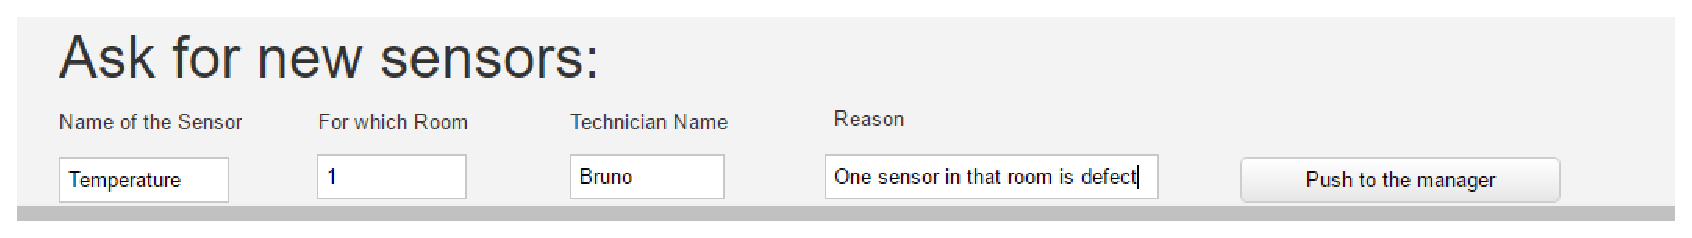
\includegraphics[width=1\textwidth]{images/AskForSensor.eps}
\end{figure} \\
2. \emph{System} pushes the information to the Manager Sensor Table on the
 managerscreen. \\
 \begin{figure}
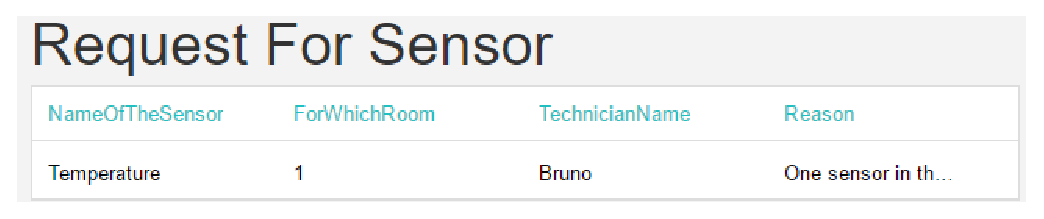
\includegraphics[width=1\textwidth]{images/requestsensor.eps}
\end{figure}
3. \emph{System.NoTA} alerts \emph{Manger} that a request has been send from
the \emph{Gardner}.\\
4. \emph{Manager} can contact now the company of the asked sensor for a new
one.\\
\item [\textbf{Extensions}]:\\
2.a  \emph{Manager} sends to the Gardner a message of
validation or not.\\
}
\end{lyxlist}

\hrule
\vspace{0.5cm}


\subsection{Sign In}
\vspace{0.5cm}
\hrule
\hfill \break
\begin{lyxlist}{PC2}
\small{
\item [\textbf{Procedure:}] SignIn
\item [\textbf{Scope:}] Identified usage of the software
\item [\textbf{Primary Actor}:] User
\item [\textbf{Secondary Actor(s)}:] Greenhouse Software GS
\item [\textbf{Goal:}] Show the user GUI to manage the garden
\item [\textbf{Level}:] User-goal level
\item [\textbf{Main~Success~Scenario}]:\\
1. \emph{User} enters a username and password combination and signs in\\
2. \emph{GS} looks up the user rights defined by the administrator\\
3. \emph{GS} now show the correct Graphical User Interface (GUI) \emph{(Gardener, Technician, Manager or Administrator)} able to control the garden.
\item [\textbf{Extensions}]:\\
1.a Wrong username and password combination\\
\hspace*{0.5cm} 1.a.1 \emph{GS} notifies the \emph{User} that the entered information are wrong\\
\hspace*{0.5cm} \textbf{procedure recontinues at step 1}
}
\end{lyxlist}
\hrule
\vspace{0.5cm}



\subsection{Adding data}
\vspace{0.5cm}
\hfill \break
\hrule
\begin{lyxlist}{PC3}
\small{
\item [\textbf{Procedure:}] Adding data
\item [\textbf{Scope:}] Adding data to a datalist
\item [\textbf{Primary Actor}:] Manager
\item [\textbf{Secondary Actor(s)}:] Greenhouse Software GS
\item [\textbf{Goal:}] Adding a task to the schedule
\item [\textbf{Level}:] User-goal level
\item [\textbf{Main~Success~Scenario}]:\\
1. \emph{User} presses the “add” button\\
2. \emph{GS} adds the task to the schedule\\
}
\end{lyxlist}
\hrule
\vspace{0.5cm}








\section{Mono-procedures}
Mono-procedures must be grouped by actors.


\subsection{MyActor1}

\subsubsection{MyProcedure1MyActor1}
\ldots

\subsubsection{MyProcedure2MyActor1}
\ldots


\subsection{My-Actor2}

\subsubsection{MyProcedure1MyActor2}
\ldots

\subsubsection{MyProcedure2MyActor2}
\ldots














